\documentclass[12pt,a4paper]{report}

\usepackage[margin=2.5cm]{geometry}
\usepackage{graphicx}
\usepackage{booktabs}
\usepackage{tabularx}
\usepackage{array}
\usepackage{amsmath}
\usepackage{amssymb}
\usepackage{listings}
\usepackage[table]{xcolor}
\usepackage{setspace}
\usepackage{float}
\usepackage{enumitem}
\usepackage[ruled,vlined]{algorithm2e}
\usepackage[hidelinks]{hyperref}

\onehalfspacing
\setlength{\parindent}{0pt}
\setlength{\parskip}{0.6em}

\newcolumntype{Y}{>{\raggedright\arraybackslash}X}
\newcolumntype{Z}{>{\centering\arraybackslash}X}
\newcolumntype{L}[1]{>{\raggedright\arraybackslash}p{#1}}
\newcolumntype{C}[1]{>{\centering\arraybackslash}p{#1}}
\newcolumntype{B}[1]{>{\bfseries\raggedright\arraybackslash}p{#1}}

\newcommand{\standardtable}{%
    \rowcolors{2}{gray!6}{white}%
    \renewcommand{\arraystretch}{1.25}%
}
\newcommand{\standardtableend}{%
    \rowcolors{2}{}{}%
    \renewcommand{\arraystretch}{1}%
}
\newcommand{\standardtablehead}[1]{%
    \toprule\rowcolor{gray!22}#1\\\midrule%
}

\lstset{
    basicstyle=\ttfamily\small,
    breaklines=true,
    frame=single,
    columns=fullflexible,
    showstringspaces=false
}

\begin{document}

\pagenumbering{roman}
\tableofcontents
\listoffigures
\listoftables

\clearpage
\pagenumbering{arabic}

\chapter*{General Introduction}
\addcontentsline{toc}{chapter}{General Introduction}

The financial relationship between large corporate actors and their commercial partners has become one of the most sensitive points in modern banking operations. Suppliers often need liquidity before invoice maturity. Buyers seek longer payment terms without weakening their commercial network. Banks, positioned between these two forces, must transform trade data into controlled financing operations while preserving security, traceability, regulatory discipline, and operational speed. This is the business terrain in which Supply Chain Finance operates.

Supply Chain Finance, commonly referred to as SCF, covers a family of financing mechanisms designed to optimize working capital across a commercial chain. Its purpose is not limited to granting credit. It restructures the timing of cash movement between anchors, counterparties, and financial institutions. In an SCF program, a bank can rely on the commercial strength of an anchor, the validity of invoices or other underlying instruments, and a set of negotiated rules to provide financing to suppliers, buyers, or distributors. Trade Finance completes this picture by addressing broader instruments and documentary operations linked to commercial exchange. Together, these domains form a demanding digital environment: the system must understand business roles, legal documentation, product definitions, fee rules, approval workflows, and transaction lifecycles.

This end-of-studies internship took place at Adria, from February 2026 to July 1st, 2026, within the Supply Chain Finance Platform Team. The project was conducted in an Agile Scrum context, where development tasks were organized through Jira tickets, source code was managed with Bitbucket, and each contribution followed a pull request review process led by the technical lead. The first two weeks were dedicated to remote integration and training, with a dual focus on the business logic of the Adria architecture and the technical stack used by the team, especially Java and Spring Boot. After this onboarding period, the work continued on-site as part of the daily development rhythm of the platform.

The internship was not limited to observation or peripheral tasks. It was situated inside an active software delivery cycle. The team was working on a Supply Chain Finance and Trade Finance platform intended for banking use cases in Morocco and North Africa. The platform digitizes the financing of trade receivables and payables between corporate anchors and their counterparties, including suppliers, distributors, and SMEs. Its functional perimeter includes reverse factoring, dynamic discounting, receivables finance, payables finance, and distributor finance. These products are configured through programs that bind together an anchor, counterparties, financing limits, fees, disbursement rules, repayment rules, and governance states.

From a technical perspective, the system follows a microservices-oriented architecture built on Adria standards. These standards provide pre-configured Spring Cloud services and reusable infrastructure patterns that support new products developed inside the company. The platform includes a core SCF service, a gateway service, a foundation data library, a properties service, a registry service, a configuration service, and supporting services for audit, storage, authentication, and document conversion. The backend stack relies mainly on Spring Boot, Spring Security, JPA/Hibernate, PostgreSQL, Eureka, Spring Cloud Config, MinIO, Gotenberg, RabbitMQ, and Keycloak. The frontend is implemented as a React application using Vite, TypeScript, React Router, React Query, Axios, and a component system based on shadcn/ui and Radix UI.

Security and governance represent a major axis of the platform. Authentication is based on Keycloak and JWT tokens, while role extraction determines whether the user operates from a bank, anchor, or counterparty view. Backend access is protected through role-based authorization. Business validation follows the maker/checker principle, a common banking governance pattern where the user who creates or modifies a record cannot approve the same operation. This principle is implemented through approval statuses, pending actions, repository specifications, and rollback mechanisms based on original data snapshots. The same concern for control appears in the gateway layer, which handles request routing, antivirus scanning for uploaded documents, brute-force protection, maintenance mode, request logging, and correlation identifiers.

Within this broader platform, the academic subject of the internship is the Disbursement Module. Its development runs in parallel with the team's sprint work because the main platform had not yet reached the sprint milestone where the module would be integrated natively into the architecture. This situation shaped the project in a very concrete way. The module had to be studied, designed, and progressively prepared while the platform itself was still evolving from Sprint 2 toward Sprint 8. Functional refinement sessions with the Product Owner played a central role in this process: the business rules were discussed, diagrams were prepared, and the proposed flows were evaluated and adjusted according to the expected target architecture.

The central problem addressed by this report is therefore twofold. The first dimension is functional: how can a banking platform organize Supply Chain Finance operations in a way that reflects the realities of anchors, counterparties, invoices, programs, fees, disbursements, repayments, and approvals? The second dimension is technical: how can such a platform be implemented with a modular architecture that remains secure, maintainable, auditable, and adaptable to several banking contexts? The Disbursement Module stands at the intersection of these two dimensions because it converts validated financing intent into an operational payment flow, while depending on upstream entities such as programs, products, invoices, fee catalogues, and eligibility rules.

This report presents the internship work through six chapters. The first chapter introduces the host organization, the business context of Supply Chain Finance and Trade Finance, the project environment, and the methodology followed during the internship. The second chapter studies the global architecture and technical stack, with attention to the microservices, gateway, security, data storage, and deployment environment. The third chapter examines the SCF domain model and backend implementation, including entities, maker/checker governance, counterparty management, product definitions, program configuration, invoice upload, and transaction inquiry. The fourth chapter focuses on frontend implementation and user flows, from authentication and role-based navigation to invoice, document, early payment, and finance disbursement screens. The fifth chapter is dedicated to the Disbursement Module as the PFE project, covering its motivation, specification, design, implementation choices, and validation. The final chapter evaluates the work performed during the internship, reflects on the acquired skills, and identifies possible future improvements.

The ambition of this document is not merely to list technologies or reproduce development tasks. It aims to analyze the construction of a banking software platform as an engineering problem shaped by business constraints, security expectations, team methodology, and architectural decisions. The work described here was carried out inside a real delivery environment, with all the friction that such an environment implies: evolving requirements, sprint priorities, review cycles, integration constraints, and the need to align academic objectives with production-oriented software practices.

\chapter{Project Context and Background}
\label{chap:project_context}

\section{Introduction}
\label{sec:ch1_introduction}

This chapter situates the internship within its professional, business, and methodological environment. A technical project does not emerge from an empty space. It takes shape inside an organization, under a particular delivery model, with a business vocabulary, a set of constraints, and a rhythm imposed by real teams. The Supply Chain Finance platform developed at Adria belongs to this kind of setting: banking software, regulatory sensitivity, iterative delivery, and a domain where each functional term carries operational weight.

The chapter begins with a presentation of Adria Business \& Technology as the host organization. It then studies the general context of Supply Chain Finance and Trade Finance, since both domains explain the logic behind the platform and the place of the Disbursement Module inside it. The last part focuses on the working methodology followed during the internship: Scrum ceremonies, Jira-based task tracking, Bitbucket pull requests, technical review, tester validation, and the parallel refinement work conducted with the Product Owner.

\section{Host Organization: Adria Business \& Technology}
\label{sec:host_organization}

\subsection{Company Overview and Positioning}
\label{subsec:company_overview}

Adria Business \& Technology is a Moroccan technology company specialized in software solutions for the financial sector. Its activity is oriented toward banks and financial institutions that need to modernize their digital channels, automate internal operations, and offer secure services to corporate and retail users. The company operates in a market where reliability is not a decorative quality. A banking platform handles identity, money movement, documents, authorizations, and traces that may later be inspected by operational teams or auditors.

The internship was carried out within Adria's Supply Chain Finance Platform Team. This team works on a platform dedicated to Supply Chain Finance and Trade Finance use cases for Moroccan and North African banks. The platform aims to digitize the financing of commercial relationships between anchors, counterparties, and banks. In practical terms, this means transforming invoices, programs, product definitions, fees, eligibility rules, and approval workflows into executable software processes.

Adria's position is shaped by a double competence. The first is business-oriented: understanding banking workflows, client constraints, financial products, and governance rules. The second is technical: building distributed systems with modern frameworks, reusable company standards, secure integration layers, and maintainable user interfaces. The internship sat exactly between these two worlds. Each technical task had to make sense inside a business flow, and each business rule had to be expressed through code, data structures, APIs, or interface behavior.

\subsection{Vision, Mission, and Core Values}
\label{subsec:vision_mission}

The information available in the internship context presents Adria as a partner in banking digital transformation. Its mission can be read through the nature of its products: helping financial institutions deliver digital services that are secure, scalable, configurable, and aligned with their operational models. This orientation is visible in the platform architecture, where generic technical standards coexist with banking-specific mechanisms such as maker/checker approval, role-based access, audit, document storage, and gateway-level protection.

The company's working culture, as observed during the internship, also reflects a strong concern for review and validation. Development does not stop at committing code. A ticket is implemented, pushed to Bitbucket, submitted through a pull request, reviewed by the technical lead, adjusted when comments are raised, merged only after acceptance, then sent to testing. The chain is simple when written on paper. Inside a sprint, it demands discipline.

\subsection{Areas of Expertise}
\label{subsec:areas_expertise}

Adria's expertise can be organized around three complementary axes. The first axis is banking domain knowledge, especially digital banking, Trade Finance, payment-oriented services, and corporate banking processes. The second is software engineering methodology, expressed through Agile delivery, collaborative refinement, code review, and progressive validation. The third is technical engineering, with backend, frontend, integration, security, document management, and deployment concerns.

The Supply Chain Finance platform illustrates this combination well. The project requires knowledge of financial products such as reverse factoring and receivables finance, but it also requires an architecture able to route requests through a gateway, validate JWT tokens, store business entities in PostgreSQL, keep documents in MinIO, convert documents through Gotenberg, and expose typed frontend services to a React application. The domain and the stack are inseparable here.

\subsection{Information Sheet}
\label{subsec:information_sheet}

Table~\ref{tab:adria_information_sheet} summarizes the company information made available through the project guide and internship context.

\begin{table}[H]
    \centering
    \caption{Adria Business \& Technology information sheet}
    \label{tab:adria_information_sheet}
    \standardtable
    \begin{tabularx}{\textwidth}{B{0.34\textwidth} Y}
        \standardtablehead{\textbf{Item} & \textbf{Information}}
        Company name & Adria Business \& Technology \\
        Chief Executive Officer and founder & Mr. BEKKAR Rachid \\
        Legal structure & Limited Liability Company with Sole Proprietor \\
        Business sector & IT consulting and financial software services \\
        Commercial register ID & 276409 \\
        Company size & 51--200 employees \\
        Date of establishment & 2013 \\
        Address & Shore 26, 2nd Floor, Casa Nearshore Park, Casablanca, Morocco \\
        Contact & contact@adria-bt.com \\
        Website & www.adria-bt.com \\
    \end{tabularx}
    \standardtableend
\end{table}

\subsection{Products and Services Portfolio}
\label{subsec:products_services}

The example report supplied in the input material identifies several product families associated with Adria's activity: mobile and web banking, mobile wallet, cash management, electronic signature, and Trade Finance solutions. These products share a common direction. They move banking operations from fragmented manual channels toward digital workflows where the client, the bank officer, the back office, and the administration layer can act through controlled interfaces.

The Supply Chain Finance platform belongs to this broader portfolio of financial software. It extends the same logic to corporate financing operations. Rather than treating invoices, counterparties, documents, fees, and approvals as scattered files or manual exchanges, the platform brings them into a structured system where operations can be created, reviewed, approved, queried, and traced.

\subsection{Organizational Structure}
\label{subsec:organizational_structure}

The company structure described in the guide material places general management above several functional divisions, including delivery, integration and support, research and development, commercial activity, and human resources administration. For the internship, the most relevant part of this structure was the technical delivery environment. The intern was not detached from the project team. Work was performed within the Supply Chain Finance Platform Team, under the supervision of a technical lead and in coordination with the Product Owner during refinement activities.

This organizational setting matters because it explains how decisions were made. Functional questions were clarified with the Product Owner. Implementation choices were reviewed by the technical lead. Validation was transferred to testing after merge. The internship therefore exposed the student to the full chain of a real software delivery organization, not only to isolated development.

\subsection{Strategic Partnerships and Clientele}
\label{subsec:partnerships_clientele}

The available guide material presents Adria as a company collaborating with banks and financial institutions across several countries in Africa, Europe, and Asia. In the context of this report, the point is not to reproduce a marketing catalogue. What matters technically is that such a client base imposes configurability. Banking platforms cannot be rigid copies of a single deployment. They often need profiles, branding, authentication settings, environment variables, data isolation rules, and integration options adapted to each institution.

This expectation appears in the project context through Adria standards and environment-specific configurations. New products rely on pre-configured Spring Cloud services and reusable infrastructure patterns. The platform is therefore designed not only for one development environment, but for a banking product line where different institutional contexts may require different configuration layers.

\section{General Context of the Project}
\label{sec:general_project_context}

\subsection{Supply Chain Finance: Domain Overview}
\label{subsec:scf_overview}

Supply Chain Finance is a set of financing techniques used to improve working capital across commercial relationships. It addresses a frequent tension: suppliers may need early liquidity, while buyers may prefer to preserve longer payment terms. The bank intervenes by transforming approved commercial obligations, often invoices or equivalent instruments, into financing opportunities under a controlled program.

The SCF ecosystem is built around three main actors. The anchor is usually a large buyer or seller whose commercial strength structures the program. The counterparty may be a supplier, buyer, distributor, SME, or corporate partner linked to the anchor. The bank configures the program, validates conditions, finances eligible operations, and supervises the lifecycle. Figure~\ref{fig:scf_ecosystem} presents this ecosystem in a simplified form.

\begin{figure}[H]
    \centering
    
\includegraphics[width=\textwidth, keepaspectratio]{images/ch1_scf_ecosystem.png}
    \caption{Supply Chain Finance ecosystem}
    \label{fig:scf_ecosystem}
\end{figure}

The financing logic depends on the product type. In reverse factoring, the supplier can receive early payment based on the buyer's approved invoice. In dynamic discounting, early payment may be linked to discount rules that vary according to timing. Receivables finance and payables finance address different sides of the commercial obligation. Distributor finance extends the logic toward downstream distribution networks. The platform described in the internship context supports these product families through reusable product definitions and concrete program configurations.

The two following illustrative flows, provided in the project material, make this distinction easier to read. Receivables finance is supplier-centered: the seller seeks financing against receivables owed by a buyer. Payables finance is buyer-centered: the buyer's approved obligations allow suppliers to receive early payment from the finance provider.

\begin{figure}[H]
    \centering
    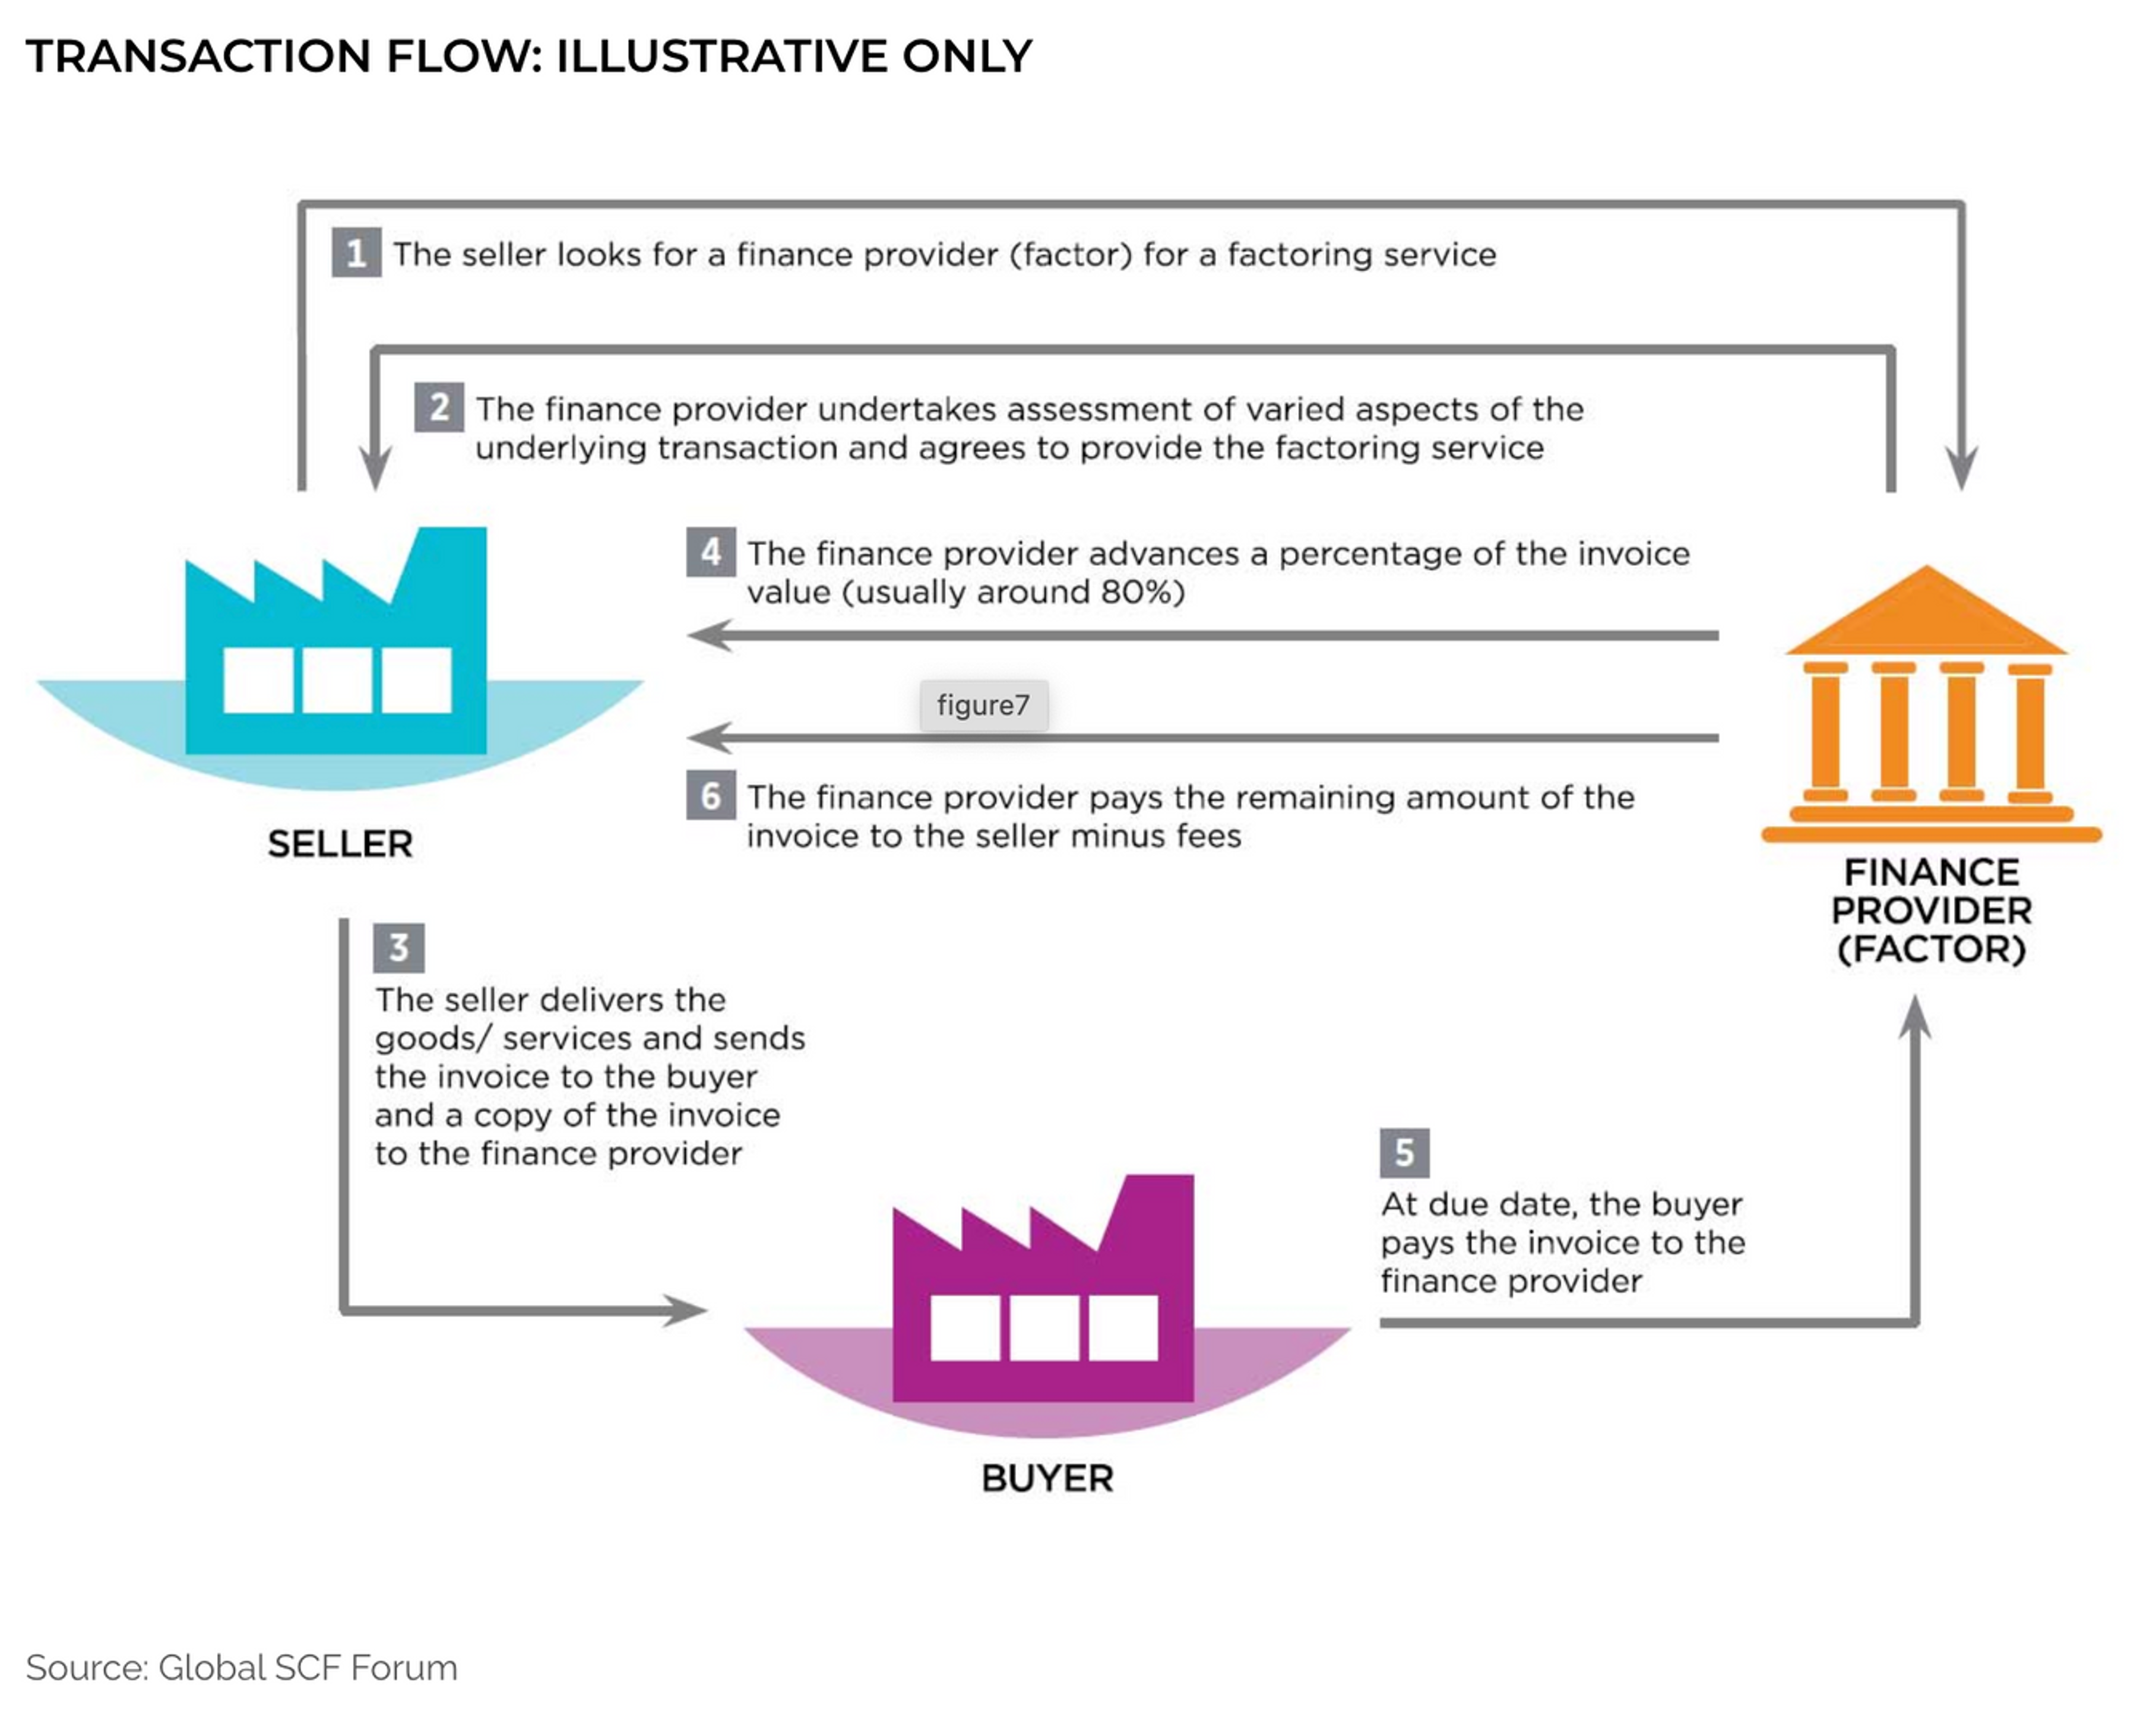
\includegraphics[width=0.88\textwidth, keepaspectratio]{images/scf_receivable_finance_transaction_flow.png}
    \caption{Illustrative transaction flow for receivables finance}
    \label{fig:ch1_receivable_finance_transaction_flow}
\end{figure}

\begin{figure}[H]
    \centering
    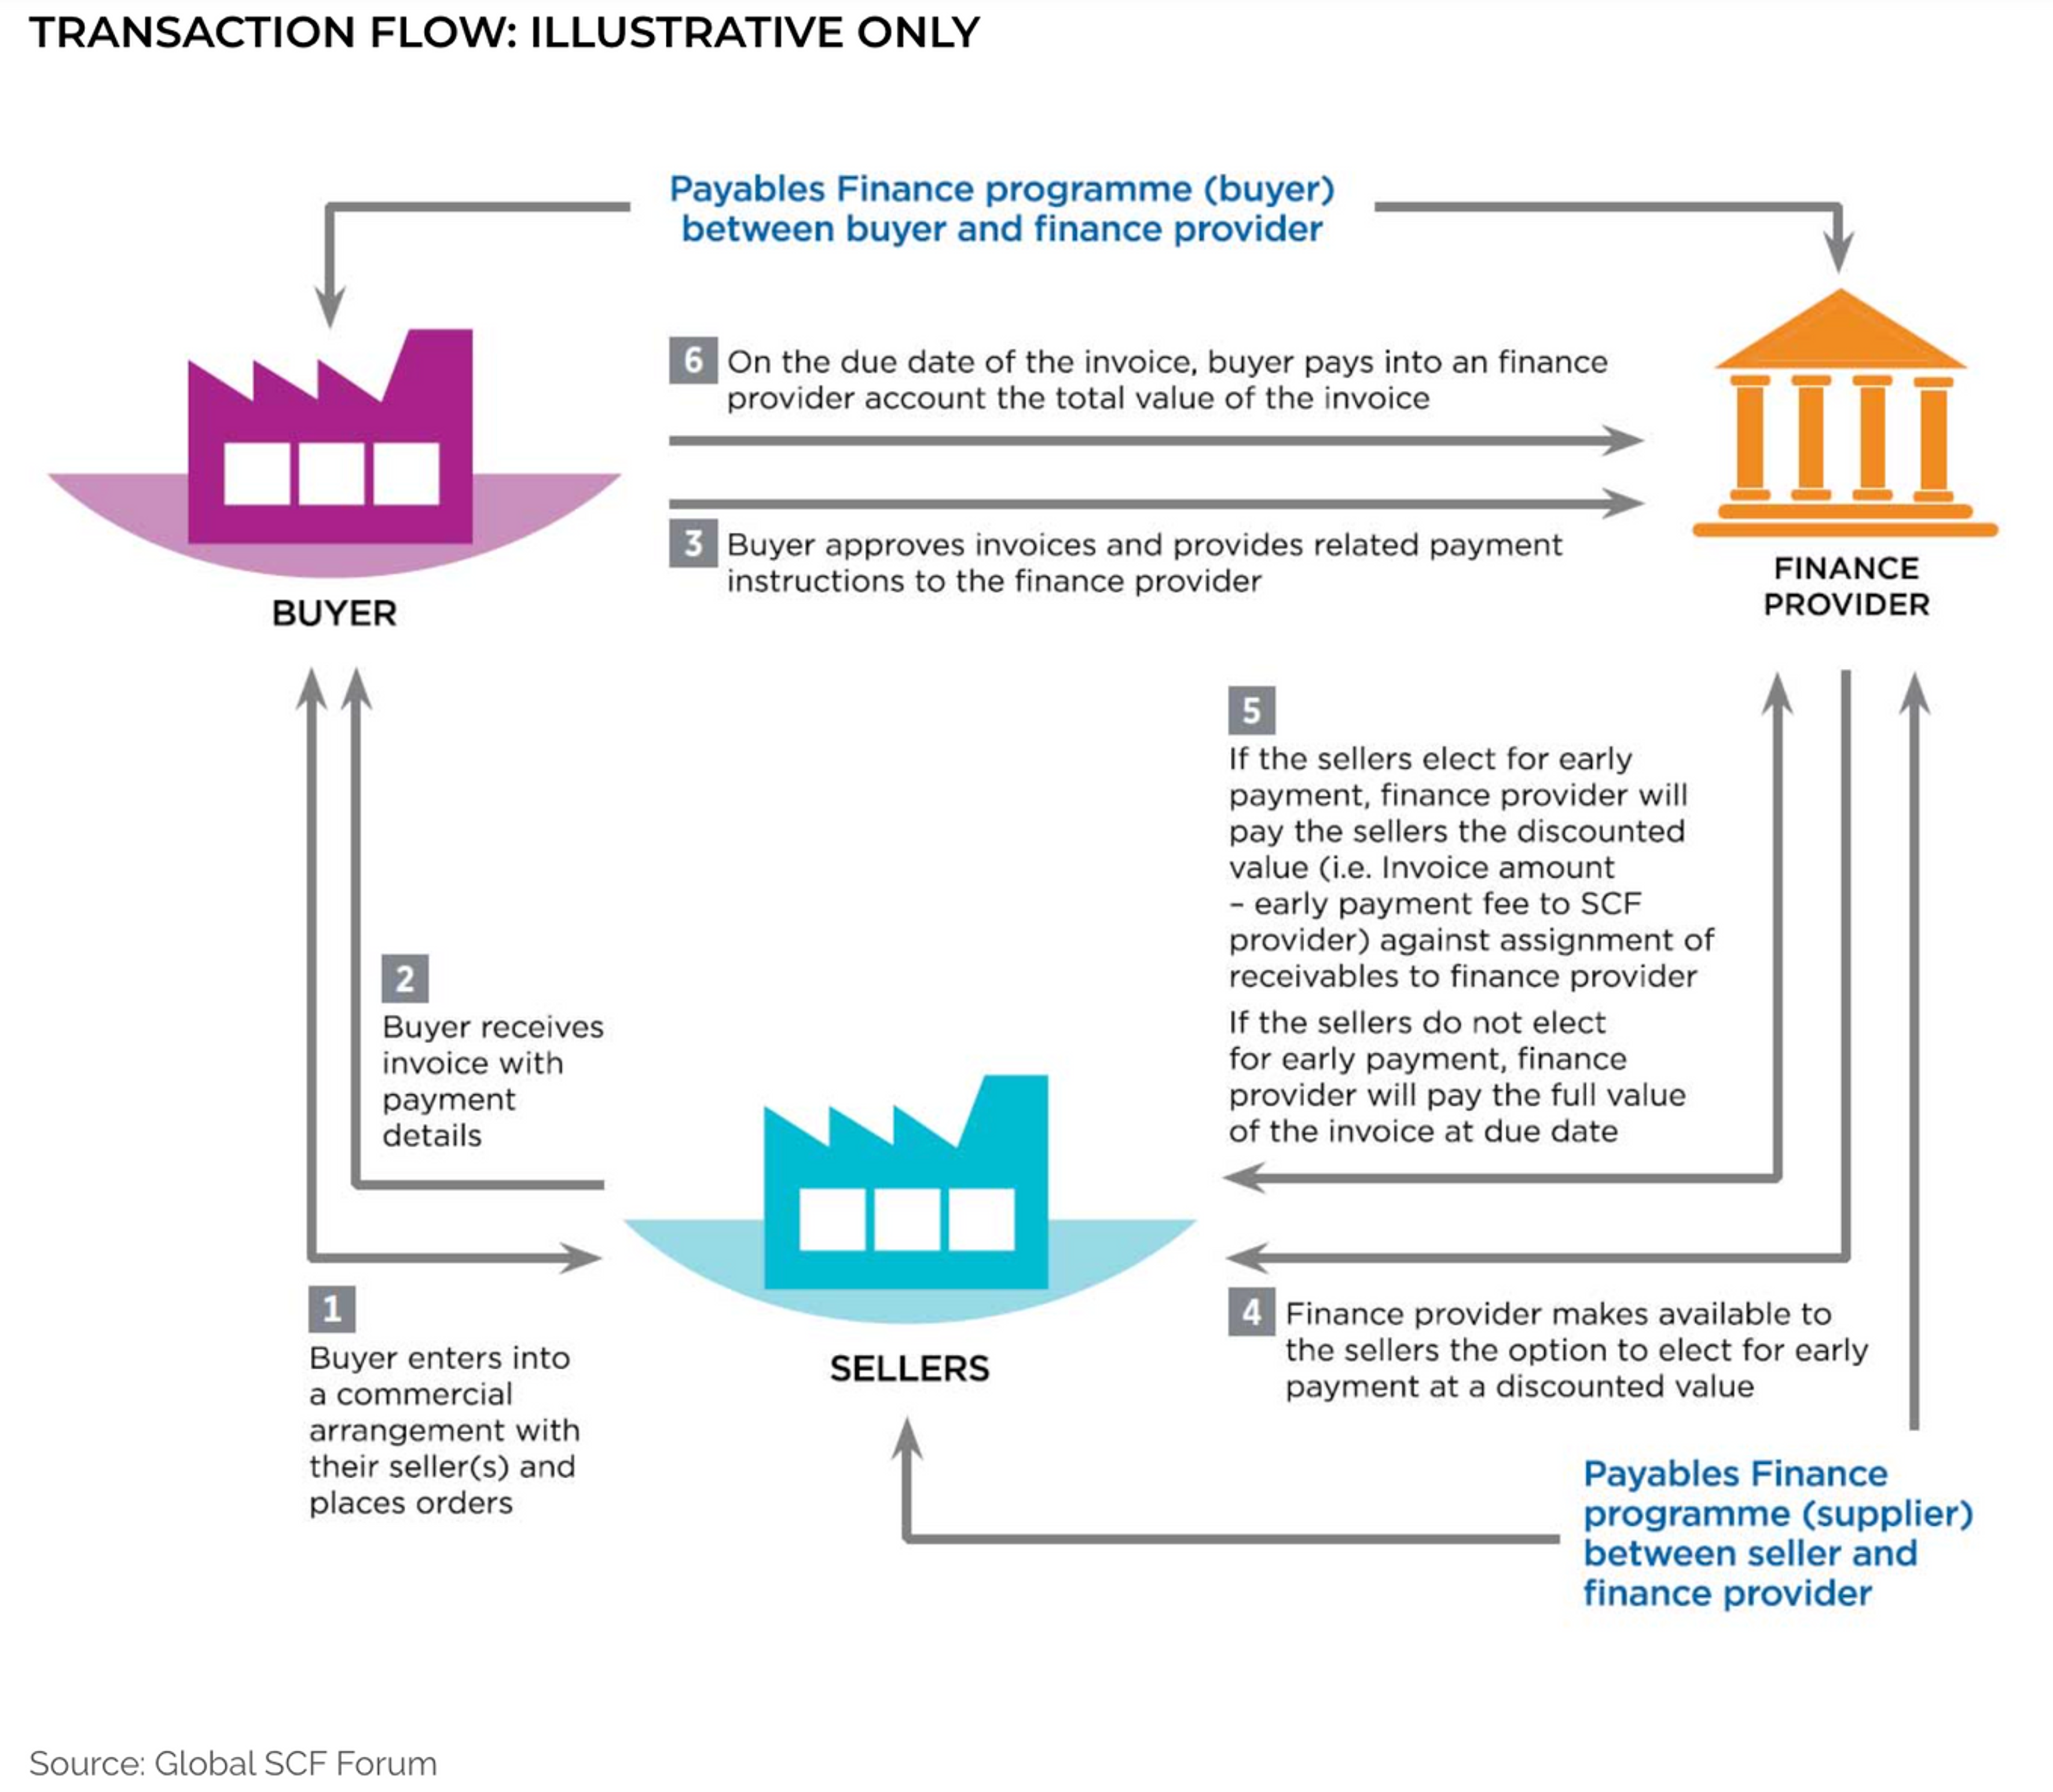
\includegraphics[width=0.88\textwidth, keepaspectratio]{images/scf_payable_finance_transaction_flow.png}
    \caption{Illustrative transaction flow for payables finance}
    \label{fig:ch1_payable_finance_transaction_flow}
\end{figure}

\subsection{Trade Finance as a Complementary Domain}
\label{subsec:trade_finance}

Trade Finance is broader than SCF. It covers financial instruments and documentary mechanisms used to secure commercial exchanges, including purchase orders, bills of exchange, promissory notes, and letters of credit. The SCF platform context explicitly references Trade Finance because the two domains share several operational concerns: document handling, counterparty identification, validation of underlying instruments, transaction tracking, and governance.

This overlap explains why the project cannot be reduced to a simple invoice screen. It needs a business model capable of representing products, programs, anchors, counterparties, documents, cashflows, fees, statuses, and approval operations. Even when the user interface appears straightforward, the underlying model remains dense.

\subsection{Problem Statement: Why Digitizing SCF and Trade Finance}
\label{subsec:problem_statement}

The digitization of SCF and Trade Finance responds to several operational problems. Manual handling of invoices and financing requests makes the process slower and more exposed to errors. Scattered documents complicate traceability. Approval decisions become harder to audit when they are not attached to structured records. Product rules may be inconsistently applied if they live outside the system. For banks, these weaknesses are not minor inconveniences; they can affect risk control, client service, and operational visibility.

The platform addresses these issues by moving business operations into a structured digital workflow. Counterparties are onboarded with bank accounts and documents. Product definitions create reusable templates. Programs bind anchors, counterparties, finance limits, fee catalogues, cashflows, disbursement methods, and repayment methods. Maker/checker governance ensures that sensitive records are not approved by their own creator. Gateway-level filters add protection around uploaded files, login attempts, maintenance mode, and request traceability.

\subsection{Proposed Solution and Platform Ambition}
\label{subsec:proposed_solution}

The proposed solution is a Supply Chain Finance and Trade Finance platform built around a modular SCF business service and the Adria technical standard. Its ambition is to provide banks with a configurable environment for managing corporate financing programs and their related operations. The SCF service groups the main business modules, while supporting services handle reference data, runtime properties, gateway routing, discovery, configuration, audit, storage, and document conversion. The frontend provides role-based access to dashboards, master setup, counterparty onboarding, invoice upload, transaction inquiry, document inquiry, early payment, and finance disbursement flows.

The project context makes an important distinction between product and program. A product definition is a reusable template such as reverse factoring or receivables finance. A program is a concrete instance linked to an anchor, counterparties, currency, dates, limits, fees, disbursement rules, and repayment rules. This distinction is one of the intellectual hinges of the platform: it separates reusable banking product design from the operational configuration used for a specific business relationship.

\subsection{Multi-Bank and Configuration Strategy}
\label{subsec:multi_bank_strategy}

The initial context file contained a broad statement about multi-tenant ambition and audit routing. A correction then clarified the scope that should be retained for this report: Adria teams follow internal standards when starting a new product. These standards include pre-configured Spring Cloud services and multiple environment configurations. Some advanced components, such as the audit service, are handled by another team and remain outside the intern's direct scope, even if they influence the general platform environment.

This distinction is important. The report can analyze the presence of standards without pretending that every standard service was designed or implemented during the internship. The relevant conclusion is more measured: the SCF platform is developed inside an ecosystem of reusable Adria services, and this ecosystem encourages consistency across products through common configuration, gateway, discovery, and infrastructure patterns.

\section{Project Methodology and Management}
\label{sec:project_methodology}

\subsection{Agile Framework: Scrum at Adria}
\label{subsec:scrum_adria}

The internship followed an Agile Scrum methodology. The student joined the platform team during Sprint 2 and the project context indicates that the team was entering Sprint 8 at the time the notes were prepared. This means the internship unfolded across an active delivery sequence rather than a frozen specification phase. Requirements, implementation tasks, reviews, and functional discussions moved together.

Scrum gave the work a repeated rhythm. Sprint planning and task assignment defined short-term priorities. Refinement sessions clarified upcoming business needs. Development work was organized around Jira tickets. Pull requests provided a review gate before code reached the shared branch. Testing followed after merge. This rhythm is shown in Figure~\ref{fig:internship_workflow}.

\begin{figure}[H]
    \centering
    
\includegraphics[width=\textwidth, keepaspectratio]{images/ch1_internship_workflow.png}
    \caption{Daily development and validation workflow}
    \label{fig:internship_workflow}
\end{figure}

\subsection{Sprint Structure and Jira-Based Ticket Management}
\label{subsec:jira_management}

Each development task was tracked through Jira. The ticket served as a unit of coordination: it described the expected work, provided visibility inside the sprint, and made progress observable by the team. Once the implementation was finished, the code was pushed to Bitbucket and submitted through a pull request. The technical lead reviewed the changes and either requested modifications or merged the branch.

After merge, the ticket moved to the tester for verification. This sequence exposed the intern to a professional feedback loop. Code was not judged only by whether it worked locally. It had to be readable enough for review, compatible with team conventions, and acceptable for later validation. That pressure is useful. It teaches engineering habits faster than isolated exercises.

\subsection{Developer Role and Contribution Scope}
\label{subsec:developer_role}

The internship role combined daily platform tasks with the academic PFE assignment. On the team side, the work involved participation in the existing software development lifecycle, using the same tools and review process as the rest of the developers. On the academic side, the assigned project was the Disbursement Module.

The Disbursement Module was treated as parallel work because the main Supply Chain Finance platform had not yet reached the sprint milestone where this module would be natively injected into the architecture. Development and analysis therefore happened dynamically: during gaps in the sprint cycle, after assigned Jira tickets, and especially through weekly refinement discussions with the Product Owner. This arrangement gave the project a particular character. It was not a finished module dropped into an already stable platform; it was a module being shaped while the platform around it was still growing.

\subsection{Tools and Work Environment}
\label{subsec:tools_environment}

The working environment combined project management, development, version control, review, and validation tools. Table~\ref{tab:tools_environment} summarizes the tools explicitly identified in the internship context and associated guide material.

\begin{table}[H]
    \centering
    \caption{Tools and work environment}
    \label{tab:tools_environment}
    \standardtable
    \begin{tabularx}{\textwidth}{B{0.28\textwidth} Y}
        \standardtablehead{\textbf{Tool or environment} & \textbf{Role during the internship}}
        Jira & Sprint task assignment, ticket tracking, and progress visibility \\
        Bitbucket & Source code hosting, branch publication, and pull request workflow \\
        Pull request review & Technical validation by the team lead before merge \\
        Tester validation & Verification of merged tickets after development review \\
        Java and Spring Boot & Main backend development stack studied during onboarding and used by the platform \\
        React, Vite, and TypeScript & Frontend stack of the SCF application \\
        Keycloak & Identity and access management through roles and JWT tokens \\
        Docker Compose & Local infrastructure provisioning for development services \\
    \end{tabularx}
    \standardtableend
\end{table}

\subsection{Timeline and Internship Planning}
\label{subsec:timeline_planning}

The internship lasted five months, from February 2026 to July 1st, 2026. The first two weeks were dedicated to remote training. This initial phase covered the business layer of Adria's architecture and the core technical stack, especially Java and Spring Boot. After that, the work moved fully on-site and became part of the daily sprint rhythm.

Alongside the team assignments, the Disbursement Module followed a parallel design loop. Each Monday, during refinement sessions, the Product Owner explained the business concepts and requirements related to the module. Functional diagrams were then prepared and discussed. The Product Owner evaluated these diagrams, validated them when aligned with the expected architecture, or requested modifications when the flow needed correction. Figure~\ref{fig:internship_timeline} presents the main timeline.

\begin{figure}[H]
    \centering
    
\includegraphics[width=\textwidth, keepaspectratio]{images/ch1_internship_timeline.png}
    \caption{Internship timeline and parallel Disbursement Module refinement}
    \label{fig:internship_timeline}
\end{figure}

This timeline created a productive tension between delivery and analysis. The daily tasks provided exposure to the real platform: entities, endpoints, frontend modules, security rules, review comments, and testing expectations. The Disbursement Module required a more forward-looking effort, since it had to be prepared before its complete integration into the platform roadmap. Both dimensions fed each other. The platform tasks made the academic module more concrete, while the module forced a deeper reading of the SCF value chain.

\section{Conclusion}
\label{sec:ch1_conclusion}

This chapter established the environment in which the internship took place. Adria Business \& Technology was presented as a financial software company working on banking digital transformation, with the Supply Chain Finance Platform Team providing the direct professional setting. The SCF and Trade Finance context clarified the business reasons behind the platform: financing commercial relationships, structuring programs, governing approvals, managing documents, and giving banks a controlled digital workflow.

The chapter also showed that the internship was organized inside a real Agile delivery process. Jira tickets, Bitbucket branches, pull requests, technical lead review, and tester validation formed the daily development chain. The Disbursement Module, assigned as the PFE project, was developed in parallel with this chain because the platform had not yet reached its native integration sprint for that module. The next chapter moves from context to architecture. It studies the technical structure that supports the platform: microservices, Adria standards, gateway routing, security, storage, frontend architecture, and deployment infrastructure.


\end{document}
